\documentclass[crop,tikz,convert={outext=.svg,command=\unexpanded{pdf2svg \infile\space\outfile}},multi=false]{standalone}[2012/04/13]
%\usetikzlibrary{...}% tikz package already loaded by 'tikz' option
\makeatletter
\begin{document}% Created by tikzDevice version 0.12.3 on 2019-09-06 10:09:11
	% Created by tikzDevice version 0.12.3 on 2019-09-06 09:53:59
	% !TEX encoding = UTF-8 Unicode
% Created by tikzDevice version 0.12.3 on 2019-09-14 12:50:35
% !TEX encoding = UTF-8 Unicode
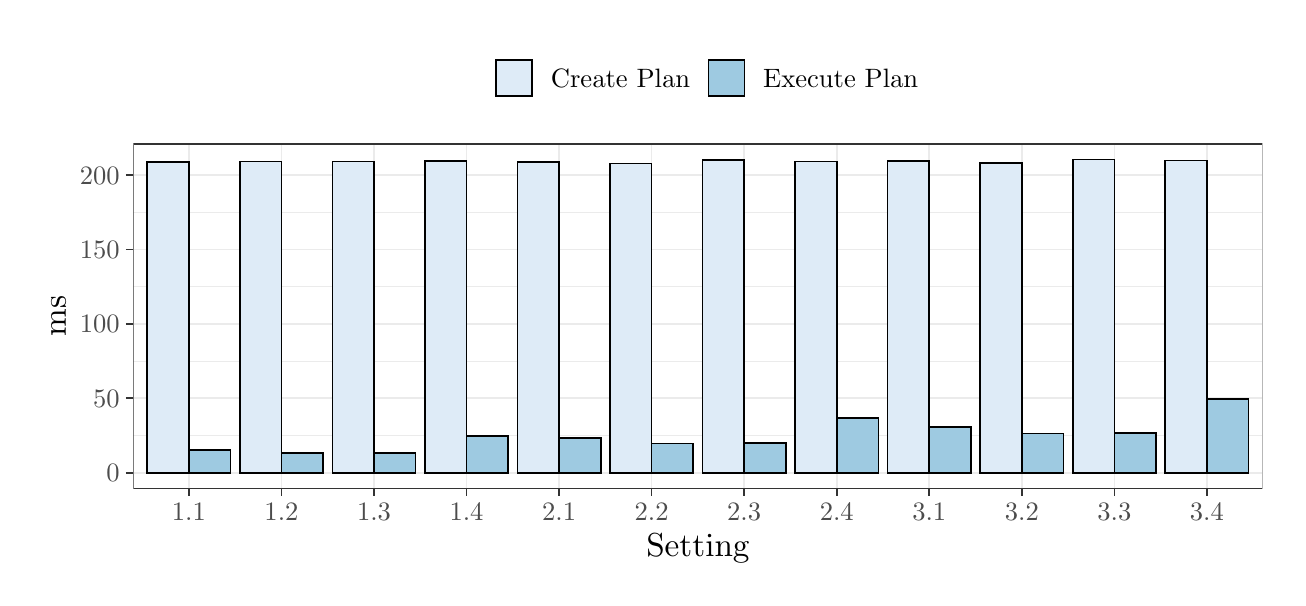
\begin{tikzpicture}[x=1pt,y=1pt]
\definecolor{fillColor}{RGB}{255,255,255}
\path[use as bounding box,fill=fillColor,fill opacity=0.00] (0,0) rectangle (451.69,198.74);
\begin{scope}
\path[clip] (  0.00,  0.00) rectangle (451.69,198.74);
\definecolor{drawColor}{RGB}{255,255,255}
\definecolor{fillColor}{RGB}{255,255,255}

\path[draw=drawColor,line width= 0.6pt,line join=round,line cap=round,fill=fillColor] (  0.00,  0.00) rectangle (451.69,198.74);
\end{scope}
\begin{scope}
\path[clip] ( 38.19, 32.28) rectangle (446.19,156.79);
\definecolor{fillColor}{RGB}{255,255,255}

\path[fill=fillColor] ( 38.19, 32.28) rectangle (446.19,156.79);
\definecolor{drawColor}{gray}{0.92}

\path[draw=drawColor,line width= 0.3pt,line join=round] ( 38.19, 51.39) --
	(446.19, 51.39);

\path[draw=drawColor,line width= 0.3pt,line join=round] ( 38.19, 78.29) --
	(446.19, 78.29);

\path[draw=drawColor,line width= 0.3pt,line join=round] ( 38.19,105.19) --
	(446.19,105.19);

\path[draw=drawColor,line width= 0.3pt,line join=round] ( 38.19,132.09) --
	(446.19,132.09);

\path[draw=drawColor,line width= 0.6pt,line join=round] ( 38.19, 37.94) --
	(446.19, 37.94);

\path[draw=drawColor,line width= 0.6pt,line join=round] ( 38.19, 64.84) --
	(446.19, 64.84);

\path[draw=drawColor,line width= 0.6pt,line join=round] ( 38.19, 91.74) --
	(446.19, 91.74);

\path[draw=drawColor,line width= 0.6pt,line join=round] ( 38.19,118.64) --
	(446.19,118.64);

\path[draw=drawColor,line width= 0.6pt,line join=round] ( 38.19,145.54) --
	(446.19,145.54);

\path[draw=drawColor,line width= 0.6pt,line join=round] ( 58.26, 32.28) --
	( 58.26,156.79);

\path[draw=drawColor,line width= 0.6pt,line join=round] ( 91.70, 32.28) --
	( 91.70,156.79);

\path[draw=drawColor,line width= 0.6pt,line join=round] (125.14, 32.28) --
	(125.14,156.79);

\path[draw=drawColor,line width= 0.6pt,line join=round] (158.59, 32.28) --
	(158.59,156.79);

\path[draw=drawColor,line width= 0.6pt,line join=round] (192.03, 32.28) --
	(192.03,156.79);

\path[draw=drawColor,line width= 0.6pt,line join=round] (225.47, 32.28) --
	(225.47,156.79);

\path[draw=drawColor,line width= 0.6pt,line join=round] (258.91, 32.28) --
	(258.91,156.79);

\path[draw=drawColor,line width= 0.6pt,line join=round] (292.35, 32.28) --
	(292.35,156.79);

\path[draw=drawColor,line width= 0.6pt,line join=round] (325.80, 32.28) --
	(325.80,156.79);

\path[draw=drawColor,line width= 0.6pt,line join=round] (359.24, 32.28) --
	(359.24,156.79);

\path[draw=drawColor,line width= 0.6pt,line join=round] (392.68, 32.28) --
	(392.68,156.79);

\path[draw=drawColor,line width= 0.6pt,line join=round] (426.12, 32.28) --
	(426.12,156.79);
\definecolor{drawColor}{RGB}{0,0,0}
\definecolor{fillColor}{RGB}{158,202,225}

\path[draw=drawColor,line width= 0.6pt,line cap=rect,fill=fillColor] ( 58.26, 37.94) rectangle ( 73.31, 46.25);
\definecolor{fillColor}{RGB}{222,235,247}

\path[draw=drawColor,line width= 0.6pt,line cap=rect,fill=fillColor] ( 43.21, 37.94) rectangle ( 58.26,150.31);
\definecolor{fillColor}{RGB}{158,202,225}

\path[draw=drawColor,line width= 0.6pt,line cap=rect,fill=fillColor] ( 91.70, 37.94) rectangle (106.75, 44.94);
\definecolor{fillColor}{RGB}{222,235,247}

\path[draw=drawColor,line width= 0.6pt,line cap=rect,fill=fillColor] ( 76.65, 37.94) rectangle ( 91.70,150.32);
\definecolor{fillColor}{RGB}{158,202,225}

\path[draw=drawColor,line width= 0.6pt,line cap=rect,fill=fillColor] (125.14, 37.94) rectangle (140.19, 45.16);
\definecolor{fillColor}{RGB}{222,235,247}

\path[draw=drawColor,line width= 0.6pt,line cap=rect,fill=fillColor] (110.09, 37.94) rectangle (125.14,150.40);
\definecolor{fillColor}{RGB}{158,202,225}

\path[draw=drawColor,line width= 0.6pt,line cap=rect,fill=fillColor] (158.59, 37.94) rectangle (173.63, 51.20);
\definecolor{fillColor}{RGB}{222,235,247}

\path[draw=drawColor,line width= 0.6pt,line cap=rect,fill=fillColor] (143.54, 37.94) rectangle (158.59,150.45);
\definecolor{fillColor}{RGB}{158,202,225}

\path[draw=drawColor,line width= 0.6pt,line cap=rect,fill=fillColor] (192.03, 37.94) rectangle (207.08, 50.48);
\definecolor{fillColor}{RGB}{222,235,247}

\path[draw=drawColor,line width= 0.6pt,line cap=rect,fill=fillColor] (176.98, 37.94) rectangle (192.03,150.23);
\definecolor{fillColor}{RGB}{158,202,225}

\path[draw=drawColor,line width= 0.6pt,line cap=rect,fill=fillColor] (225.47, 37.94) rectangle (240.52, 48.50);
\definecolor{fillColor}{RGB}{222,235,247}

\path[draw=drawColor,line width= 0.6pt,line cap=rect,fill=fillColor] (210.42, 37.94) rectangle (225.47,149.69);
\definecolor{fillColor}{RGB}{158,202,225}

\path[draw=drawColor,line width= 0.6pt,line cap=rect,fill=fillColor] (258.91, 37.94) rectangle (273.96, 48.74);
\definecolor{fillColor}{RGB}{222,235,247}

\path[draw=drawColor,line width= 0.6pt,line cap=rect,fill=fillColor] (243.86, 37.94) rectangle (258.91,150.91);
\definecolor{fillColor}{RGB}{158,202,225}

\path[draw=drawColor,line width= 0.6pt,line cap=rect,fill=fillColor] (292.35, 37.94) rectangle (307.40, 57.76);
\definecolor{fillColor}{RGB}{222,235,247}

\path[draw=drawColor,line width= 0.6pt,line cap=rect,fill=fillColor] (277.30, 37.94) rectangle (292.35,150.33);
\definecolor{fillColor}{RGB}{158,202,225}

\path[draw=drawColor,line width= 0.6pt,line cap=rect,fill=fillColor] (325.80, 37.94) rectangle (340.84, 54.41);
\definecolor{fillColor}{RGB}{222,235,247}

\path[draw=drawColor,line width= 0.6pt,line cap=rect,fill=fillColor] (310.75, 37.94) rectangle (325.80,150.67);
\definecolor{fillColor}{RGB}{158,202,225}

\path[draw=drawColor,line width= 0.6pt,line cap=rect,fill=fillColor] (359.24, 37.94) rectangle (374.29, 52.05);
\definecolor{fillColor}{RGB}{222,235,247}

\path[draw=drawColor,line width= 0.6pt,line cap=rect,fill=fillColor] (344.19, 37.94) rectangle (359.24,149.94);
\definecolor{fillColor}{RGB}{158,202,225}

\path[draw=drawColor,line width= 0.6pt,line cap=rect,fill=fillColor] (392.68, 37.94) rectangle (407.73, 52.33);
\definecolor{fillColor}{RGB}{222,235,247}

\path[draw=drawColor,line width= 0.6pt,line cap=rect,fill=fillColor] (377.63, 37.94) rectangle (392.68,151.13);
\definecolor{fillColor}{RGB}{158,202,225}

\path[draw=drawColor,line width= 0.6pt,line cap=rect,fill=fillColor] (426.12, 37.94) rectangle (441.17, 64.57);
\definecolor{fillColor}{RGB}{222,235,247}

\path[draw=drawColor,line width= 0.6pt,line cap=rect,fill=fillColor] (411.07, 37.94) rectangle (426.12,150.69);
\definecolor{drawColor}{gray}{0.20}

\path[draw=drawColor,line width= 0.6pt,line join=round,line cap=round] ( 38.19, 32.28) rectangle (446.19,156.79);
\end{scope}
\begin{scope}
\path[clip] (  0.00,  0.00) rectangle (451.69,198.74);
\definecolor{drawColor}{gray}{0.30}

\node[text=drawColor,anchor=base east,inner sep=0pt, outer sep=0pt, scale=  0.96] at ( 33.24, 34.63) {0};

\node[text=drawColor,anchor=base east,inner sep=0pt, outer sep=0pt, scale=  0.96] at ( 33.24, 61.53) {50};

\node[text=drawColor,anchor=base east,inner sep=0pt, outer sep=0pt, scale=  0.96] at ( 33.24, 88.43) {100};

\node[text=drawColor,anchor=base east,inner sep=0pt, outer sep=0pt, scale=  0.96] at ( 33.24,115.33) {150};

\node[text=drawColor,anchor=base east,inner sep=0pt, outer sep=0pt, scale=  0.96] at ( 33.24,142.24) {200};
\end{scope}
\begin{scope}
\path[clip] (  0.00,  0.00) rectangle (451.69,198.74);
\definecolor{drawColor}{gray}{0.20}

\path[draw=drawColor,line width= 0.6pt,line join=round] ( 35.44, 37.94) --
	( 38.19, 37.94);

\path[draw=drawColor,line width= 0.6pt,line join=round] ( 35.44, 64.84) --
	( 38.19, 64.84);

\path[draw=drawColor,line width= 0.6pt,line join=round] ( 35.44, 91.74) --
	( 38.19, 91.74);

\path[draw=drawColor,line width= 0.6pt,line join=round] ( 35.44,118.64) --
	( 38.19,118.64);

\path[draw=drawColor,line width= 0.6pt,line join=round] ( 35.44,145.54) --
	( 38.19,145.54);
\end{scope}
\begin{scope}
\path[clip] (  0.00,  0.00) rectangle (451.69,198.74);
\definecolor{drawColor}{gray}{0.20}

\path[draw=drawColor,line width= 0.6pt,line join=round] ( 58.26, 29.53) --
	( 58.26, 32.28);

\path[draw=drawColor,line width= 0.6pt,line join=round] ( 91.70, 29.53) --
	( 91.70, 32.28);

\path[draw=drawColor,line width= 0.6pt,line join=round] (125.14, 29.53) --
	(125.14, 32.28);

\path[draw=drawColor,line width= 0.6pt,line join=round] (158.59, 29.53) --
	(158.59, 32.28);

\path[draw=drawColor,line width= 0.6pt,line join=round] (192.03, 29.53) --
	(192.03, 32.28);

\path[draw=drawColor,line width= 0.6pt,line join=round] (225.47, 29.53) --
	(225.47, 32.28);

\path[draw=drawColor,line width= 0.6pt,line join=round] (258.91, 29.53) --
	(258.91, 32.28);

\path[draw=drawColor,line width= 0.6pt,line join=round] (292.35, 29.53) --
	(292.35, 32.28);

\path[draw=drawColor,line width= 0.6pt,line join=round] (325.80, 29.53) --
	(325.80, 32.28);

\path[draw=drawColor,line width= 0.6pt,line join=round] (359.24, 29.53) --
	(359.24, 32.28);

\path[draw=drawColor,line width= 0.6pt,line join=round] (392.68, 29.53) --
	(392.68, 32.28);

\path[draw=drawColor,line width= 0.6pt,line join=round] (426.12, 29.53) --
	(426.12, 32.28);
\end{scope}
\begin{scope}
\path[clip] (  0.00,  0.00) rectangle (451.69,198.74);
\definecolor{drawColor}{gray}{0.30}

\node[text=drawColor,anchor=base,inner sep=0pt, outer sep=0pt, scale=  0.96] at ( 58.26, 20.71) {1.1};

\node[text=drawColor,anchor=base,inner sep=0pt, outer sep=0pt, scale=  0.96] at ( 91.70, 20.71) {1.2};

\node[text=drawColor,anchor=base,inner sep=0pt, outer sep=0pt, scale=  0.96] at (125.14, 20.71) {1.3};

\node[text=drawColor,anchor=base,inner sep=0pt, outer sep=0pt, scale=  0.96] at (158.59, 20.71) {1.4};

\node[text=drawColor,anchor=base,inner sep=0pt, outer sep=0pt, scale=  0.96] at (192.03, 20.71) {2.1};

\node[text=drawColor,anchor=base,inner sep=0pt, outer sep=0pt, scale=  0.96] at (225.47, 20.71) {2.2};

\node[text=drawColor,anchor=base,inner sep=0pt, outer sep=0pt, scale=  0.96] at (258.91, 20.71) {2.3};

\node[text=drawColor,anchor=base,inner sep=0pt, outer sep=0pt, scale=  0.96] at (292.35, 20.71) {2.4};

\node[text=drawColor,anchor=base,inner sep=0pt, outer sep=0pt, scale=  0.96] at (325.80, 20.71) {3.1};

\node[text=drawColor,anchor=base,inner sep=0pt, outer sep=0pt, scale=  0.96] at (359.24, 20.71) {3.2};

\node[text=drawColor,anchor=base,inner sep=0pt, outer sep=0pt, scale=  0.96] at (392.68, 20.71) {3.3};

\node[text=drawColor,anchor=base,inner sep=0pt, outer sep=0pt, scale=  0.96] at (426.12, 20.71) {3.4};
\end{scope}
\begin{scope}
\path[clip] (  0.00,  0.00) rectangle (451.69,198.74);
\definecolor{drawColor}{RGB}{0,0,0}

\node[text=drawColor,anchor=base,inner sep=0pt, outer sep=0pt, scale=  1.20] at (242.19,  7.83) {Setting};
\end{scope}
\begin{scope}
\path[clip] (  0.00,  0.00) rectangle (451.69,198.74);
\definecolor{drawColor}{RGB}{0,0,0}

\node[text=drawColor,rotate= 90.00,anchor=base,inner sep=0pt, outer sep=0pt, scale=  1.20] at ( 13.76, 94.53) {ms};
\end{scope}
\begin{scope}
\path[clip] (  0.00,  0.00) rectangle (451.69,198.74);
\definecolor{fillColor}{RGB}{255,255,255}

\path[fill=fillColor] (157.10,167.79) rectangle (327.28,193.24);
\end{scope}
\begin{scope}
\path[clip] (  0.00,  0.00) rectangle (451.69,198.74);
\definecolor{fillColor}{RGB}{255,255,255}

\path[fill=fillColor] (168.60,173.29) rectangle (183.06,187.74);
\end{scope}
\begin{scope}
\path[clip] (  0.00,  0.00) rectangle (451.69,198.74);
\definecolor{drawColor}{RGB}{0,0,0}
\definecolor{fillColor}{RGB}{222,235,247}

\path[draw=drawColor,line width= 0.6pt,line cap=rect,fill=fillColor] (169.31,174.00) rectangle (182.35,187.03);
\end{scope}
\begin{scope}
\path[clip] (  0.00,  0.00) rectangle (451.69,198.74);
\definecolor{fillColor}{RGB}{255,255,255}

\path[fill=fillColor] (245.34,173.29) rectangle (259.79,187.74);
\end{scope}
\begin{scope}
\path[clip] (  0.00,  0.00) rectangle (451.69,198.74);
\definecolor{drawColor}{RGB}{0,0,0}
\definecolor{fillColor}{RGB}{158,202,225}

\path[draw=drawColor,line width= 0.6pt,line cap=rect,fill=fillColor] (246.05,174.00) rectangle (259.08,187.03);
\end{scope}
\begin{scope}
\path[clip] (  0.00,  0.00) rectangle (451.69,198.74);
\definecolor{drawColor}{RGB}{0,0,0}

\node[text=drawColor,anchor=base west,inner sep=0pt, outer sep=0pt, scale=  0.96] at (189.06,177.21) {Create Plan};
\end{scope}
\begin{scope}
\path[clip] (  0.00,  0.00) rectangle (451.69,198.74);
\definecolor{drawColor}{RGB}{0,0,0}

\node[text=drawColor,anchor=base west,inner sep=0pt, outer sep=0pt, scale=  0.96] at (265.79,177.21) {Execute Plan};
\end{scope}
\end{tikzpicture}
\end{document}
